%%%%%%%%%%%%%%%%%%%%%%%%%%%%%%%%%%%%%%%%%%%%
%%% WHISPERS
%%%%%%%%%%%%%%%%%%%%%%%%%%%%%%%%%%%%%%%%%%%%

\mysection{Whispers}{vulgate-whispers}

  \callout {
    Using a Whisper takes Moments; in Combat, using a Whisper is a Basic Maneuver. You don't need hands, but you need to be able to speak and move freely. You can only be wearing Light Armor, and you can't be carrying a Shield.
}


    Whispers are the hedge magic, illusion, sleight-of-hand, and minor telepathy that constitute the \mybold{Left Hand Path}.  Passed down through instruction, ancient books, and word-of-mouth, Whispers allow you to cheat \mylink{the Game}{the-game} very subtly.  Whispers are generally used by \mylink{Knaves}{trope-knave}, but \mylink{Murks}{species-murk} and \mylink{Pooka}{species-pooka} have expertise in the \mylink{Whispers of The Bride}{vulgate-whisper-the-bride} and the \mylink{Whispers of Br'er Rabbit}{vulgate-whisper-brer-rabbit}, respectively.

    Using a Whisper in Combat is a \mylink{Basic Maneuver}{combat-basic-maneuver}. Whispers require you to be able to move and act freely, so you must be unarmored or wearing \mylink{Light Armor}{gear-armor}, and you can't carry a \mylink{Shield}{gear-armor}.  Like \mylink{Secrets}{arcana-wizardry-secrets}, Whispers require verbalization; a common punishment for thieves is to cut out their tongues. You must be able to speak in order to use a Whisper.

\myimage{vulgate/Whispers1}

\cbreak


\mysubsection{The Whisper Die}{vulgate-whispers-knave}

  \formula {Whisper Try}{
    \RB : \KNAVE \PLUS \LUCK (up to +4) vs. Difficulty
  }


Your skill with a particular Whisper is indicated by your \KNAVE:

\mytable{X c}{
  \thead{Rank} & \thead{\KNAVE} \\
}{
  Untrained  & 1 \\
  Apprentice & d4  \\
  Footpad & d6  \\
  Sharper & d8  \\
  Master & d10  \\
}

\mybold{You may use your \LUCK to affect your \KNAVE roll, but it can never provide more than a +4 Modifier.}


    Rolling your \KNAVE should only be required by the Arbiter if the difference between success and failure would be interesting, or when the attempt shouldn't be an automatic success.  If you are "Untrained" in one of the Whispers, it means you know only the bare details; you would only succeed if the difference between success and failure would be uninteresting or an automatic success. You may buy additional ranks in a Whisper when you \mylink{advance in level}{advancement}.

\mysubsection{Difficulty}{vulgate-whispers-difficult}

 If the Arbiter decides the roll is required, she will set a Difficulty for the roll (a number between 2 and 9; examples are below). You must make a \RB{\KNAVE} try against the Difficulty number.

 Determining the Difficulty of a task is up to the Arbiter. Some examples that might help you calibrate:


  \mybold{Climbing:} Every 10m should be a point of difficulty.  Add a point if the object being climbed is particularly slippery, it's windy, or if the Knave is encumbered or injured; subtract a point if the Knave has rope or climbing gear, or strips off equipment to make climbing easier. \myital{\mylink{Whispers of Anne Bonny}{vulgate-whisper-anne-bonny}}

   \mybold{Disguise and Forgery:}   Using minor details to disguise yourself as a stranger, or lying to a kid might be a 2; changing your gender or species, or forging an arrest warrant, might be a 4 or 5; pretending you're someone famous might be a 7; lying to a Sphinx, forging an Article of War, or fooling a close friend might be a 9. \myital{\mylink{Whispers of Anne Bonny}{vulgate-whisper-anne-bonny}}

    \mybold{Picking Pockets:} Picking the pocket of a common yokel in a crowded street might be a 2; stealing the keys from a guard's belt might be a 5; palming a card in a game with demons might be a 7; stealing the rings from the king's finger when you kiss his hand might be a 9. \myital{\mylink{Whispers of Br'er Rabbit}{vulgate-whisper-brer-rabbit}}

      \mybold{Locks:} A common lock on a blacksmith's shop might be a 2; your hands bound with rope might be a 4; a jeweler's lockbox in a Large settlement might be a 5; slipping free of manacles might be a 6;  an item locked by the Lock spell might be a 7; the lock on the Gates of Hell would be a 9. \myital{\mylink{Whispers of Sun Wukong}{vulgate-whisper-sun-wukong}}

       \mybold{Traps:} assign two Difficulties - the Difficulty of \mybold{finding} the trap and the Difficulty of \mybold{disarming} a trap.  A hunter's snare or goblin trap might be a 2 or 3; a elaborate Rube Goldberg trap in a mummy's tomb might be a 5; an invisible tripwire that triggers an explosion might be a 7; a trap designed by an Grimtooth might be a 9. \mylink{Inscribed Sigils}{research-inscription} can also be erased with the Whispers of Sun Wukong. \mylink{Novice Sigils}{sigils-novice} are a 3, \mylink{Warlock Sigils}{sigils-warlock} are a 6, and \mylink{Archmage Sigils}{sigils-archmage} are a 9. \myital{\mylink{Whispers of Sun Wukong}{vulgate-whisper-sun-wukong}}
  
    \mybold{Sneaking:} Assign a point of difficulty for each \HD of a Monster.  Add a point if the area is well lit; add another point if the Knave is trying to slip past guards or someone looking for them.  Subtract a point for dark areas or distractions. A crowded room or shadowy street might be a 2 or 3; through a guarded doorway lit by torches might be a 6; hiding in someone's shadow in a well lit room might be a 9. 
    \myital{\mylink{Whispers of The Bride}{vulgate-whisper-the-bride}}

\cbreak

\begin{center}

\includegraphics[scale=.4]{vulgate/Whisper3}
\end{center}

    \example {
      Flink Lighthand is a Footpad in the Whispers of Sun Wukong with a d6 \KNAVE and a d6 \LUCK.  Creeping down a crypt hallway he peeks through the broken door of an antechamber, and sees the glint of gold at the far end.  Flink's sixth-sense is tingling though, and he asks the Arbiter if he sees any traps in here.  The Arbiter knows there's a cunning poisoned spear trap in the room and assigns a Target of 4/2 to it (4 to find it and 2 to disarm it).  Flink rolls his \KNAVE and gets a 4 - he smells a whiff of tarantula venom in the air, and the large flagstone just inside the door doesn't look right.  Bending close to the flagstone, Flink whispers to it and asks it to lock in place.  He rolls again ... and gets a 1!  Thinking quickly, Flink rolls his \LUCK and rolls a 4.  He adds 4 to his roll, making it a 5.  Lucky break - he mixed up the words of the Whisper, but it worked out better than he hoped. 

    \myskip

     Later, Flink finds himself in a spot where he has to climb a rocky cliff to continue his journey.  Flink is "Untrained" in the Whispers of Anne Bonny, but the Arbiter decides that the difference between success and failure isn't interesting at this point of the adventure (she'd rather get him to the surprises she has on the other side!).  Flink's natural ability as a Knave is enough for him to scamper up the rock face.  If the Arbiter felt that this was difficult enough to not be automatic, Flink could still roll his \LUCK and add it to his rank of 1 (Untrained) to try to get up the wall...

    }



\newpage


    \mysubsection{Whispers of Anne Bonny}{vulgate-whisper-anne-bonny}

    Also known as The Swashbuckler, Anne Bonny's instructions show the ways to scale impenetrable fortresses, icy cliffs, and wizard's towers; swing from ropes and vines; disguise yourself to escape patrolling soldiers or to get past armed guards; and forge documents to start wars or gain access to restricted areas. 

    \mysubsection{Whispers of Br'er Rabbit}{vulgate-whisper-brer-rabbit}

    Br'er Rabbit (The Curious) knows a thing or two about tight squeezes.  His Whispers can help you remove items from pockets without anyone seeing; perform sleight-of-hand, ventriloquism, and distraction to befuddle your marks; escape from ropes and manacles; and cast spells from \mylink{Fetishes}{fetishes}. 

    When casting spells from a Fetish, you roll your single \KNAVE for the spell instead of a Blood Die. If you are "Untrained" (a value of 1) you can't read any spells from Fetishes.

    \mysubsection{Whispers of Sun Wukong}{vulgate-whisper-sun-wukong}

    Sun Wukong is known as The Thief.  His teachings show the secret ways of hiding things on your person so they are difficult to find; uncovering and understanding the mechanisms of traps, snares, and Inscribed Sigils (see "Traps" above) and chiding them into disarming themselves; and opening locked chests, doors, and prisons. 


    \mysubsection{Whispers of The Bride}{vulgate-whisper-the-bride}

    The Bride is known by many names, none of them spoken aloud:  Lady Death, the Banshee, the Viper, etc.  Education in the Whispers of the Bride teaches you the mental tricks, hypnotism, and observation necessary to sneak past (or behind) people without them noticing you, to silence the clink of coins in your pocket and the sound of your breath and heartbeat. In addition, the Bride teaches you the finer points of committing \mylink{Murder}{vulgate-whispers-murder}, provided you get \mylink{the Drop}{combat-drop} (including if you are "Untrained" in this Whisper).


  \myimage{vulgate/Whispers2}



    \myhighlight{Murder}{vulgate-whispers-murder}

    If you get \mylink{The Drop}{combat-drop} on someone, you can attempt a Murder.  Murder can only be performed at Close range with a Shortsword, Dagger, Club, or Hand Axe (though see the \mylink{Virtue: Deadeye}{knave-virtue-deadeye}).  Make a standard Attack \RO; if you hit, pick \mybold{one} of the following attacks:

    \callout {
      \mybullet {
        \item \mybold{Cautious:}  You automatically deal maximum damage and \mylink{Crit}{combat-crits-and-fumbles} (meaning your total damage is \MAX + 4). Any weapon.
        \item \mybold{Reckless:}  You do 3d6 damage. Any weapon.
        \item \mybold{Bloody:}  You roll damage normally, but the Monster is also \mylink{Bleeding}{effect-bleeding}. Stabbing weapons only.
        \item \mybold{Waylaying:}  You can either roll damage and the Monster is \mylink{Woozy}{effect-woozy}, or do no damage and the Monster must Save or be \mylink{Knocked Out}{effect-knocked-out}.  Bashing weapons only.
      }
    }

   Murder is a \mylink{Combat Action}{combat-combat-actions}, so it can't be combined with other Combat Actions (like Florentine). Damage bypasses any Armor if applicable (you slip the blade between the Monster's scales / plate mail / chink in carapace). Once you commit a Murder, you no longer have the Drop unless you're able to get out of sight again. Note that Monsters who are Amorphous or immune to surprise cannot be Murdered. 


\end{multicols*}

  \example {
    Deego Foxears (3rd Level Knave with the rank of Footpad (d6) in Whispers of The Bride) and Stalwart Hamhands (a 3rd Level Sellsword) come around the corner and surprise a clutch of three Ghouls and a necromancer standing at an altar.  The ghouls are Close and the necromancer is Nearby.  The Arbiter rules the ghouls and necromancer are surprised, so Deego has The Drop.  He tries his Attack \RO and succeeds.  He's armed with a Shortsword and opts to attack "Cautiously".  He deals 10 damage (6 for the sword + 4 damage) and stabs a ghoul through the heart before it can react. Stalwart steps up behind him and guts another ghoul with his polearm.  The single remaining Ghoul is under the sway of the necromancer, so the Arbiter decides not to roll \mylink{Morale}{monster-morale} - it will stay and fight to the death.

    \myskip

    Deego and Stalwart roll Init - Deego rolls well over 20, Stalwart less so (he's wearing plate mail).  Deego takes the opportunity to duck into the shadows to try to get the Drop on the necromancer. The Arbiter gives the difficulty a 3 (2 for the ghoul's \HD; an extra 1 because the ghoul is Close and aware Deego's there, but he's mostly focused on the huge armored guy with a polearm; and no modifier for the necromancer, who's completely absorbed in his ritual). Deego makes a \RBTRY{\KNAVE}{3} try with his d6 and gets a 5; he slips out of view.  The Ghoul attacks Stalwart and hits, but Stalwart is able to absorb the damage with his Grit - just a glancing blow.  The necromancer seems to be trying to finish his ritual and doesn't make a move.  It's Stalwart and Deego's turn; Deego takes another Maneuver Action to sneak Nearby (right behind the necromancer), while Stalwart engages the remaining ghoul.  Depending on how Init goes the next Moment, Deego will be able to take a Combat Action, and hopefully stop the wizard from releasing some eldritch horror ...
  }

\begin{center}
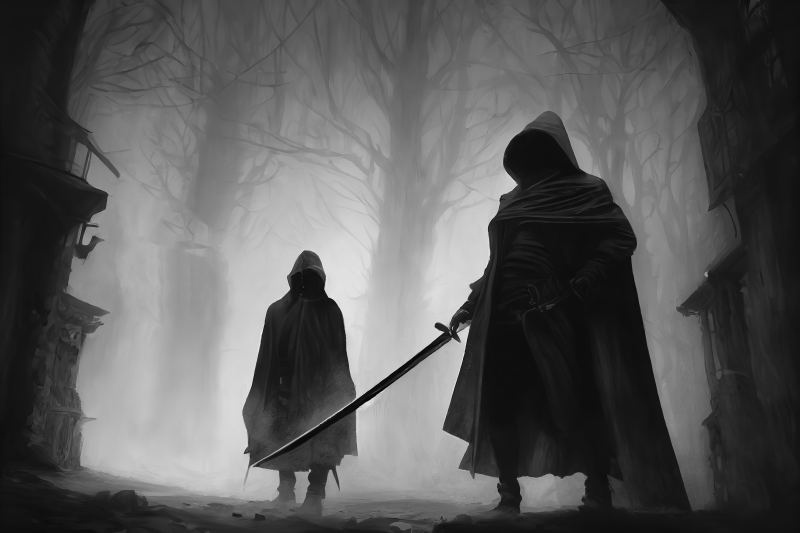
\includegraphics[scale=.5]{vulgate/Whispers4}
\end{center}

\begin{multicols*}{2}


